% Options for packages loaded elsewhere
\PassOptionsToPackage{unicode}{hyperref}
\PassOptionsToPackage{hyphens}{url}
%
\documentclass[
]{article}
\usepackage{amsmath,amssymb}
\usepackage{lmodern}
\usepackage{iftex}
\ifPDFTeX
  \usepackage[T1]{fontenc}
  \usepackage[utf8]{inputenc}
  \usepackage{textcomp} % provide euro and other symbols
\else % if luatex or xetex
  \usepackage{unicode-math}
  \defaultfontfeatures{Scale=MatchLowercase}
  \defaultfontfeatures[\rmfamily]{Ligatures=TeX,Scale=1}
  \setmainfont[]{SourceSansPro}
\fi
% Use upquote if available, for straight quotes in verbatim environments
\IfFileExists{upquote.sty}{\usepackage{upquote}}{}
\IfFileExists{microtype.sty}{% use microtype if available
  \usepackage[]{microtype}
  \UseMicrotypeSet[protrusion]{basicmath} % disable protrusion for tt fonts
}{}
\makeatletter
\@ifundefined{KOMAClassName}{% if non-KOMA class
  \IfFileExists{parskip.sty}{%
    \usepackage{parskip}
  }{% else
    \setlength{\parindent}{0pt}
    \setlength{\parskip}{6pt plus 2pt minus 1pt}}
}{% if KOMA class
  \KOMAoptions{parskip=half}}
\makeatother
\usepackage{xcolor}
\usepackage[margin=1in]{geometry}
\usepackage{graphicx}
\makeatletter
\def\maxwidth{\ifdim\Gin@nat@width>\linewidth\linewidth\else\Gin@nat@width\fi}
\def\maxheight{\ifdim\Gin@nat@height>\textheight\textheight\else\Gin@nat@height\fi}
\makeatother
% Scale images if necessary, so that they will not overflow the page
% margins by default, and it is still possible to overwrite the defaults
% using explicit options in \includegraphics[width, height, ...]{}
\setkeys{Gin}{width=\maxwidth,height=\maxheight,keepaspectratio}
% Set default figure placement to htbp
\makeatletter
\def\fps@figure{htbp}
\makeatother
\setlength{\emergencystretch}{3em} % prevent overfull lines
\providecommand{\tightlist}{%
  \setlength{\itemsep}{0pt}\setlength{\parskip}{0pt}}
\setcounter{secnumdepth}{-\maxdimen} % remove section numbering
\ifLuaTeX
  \usepackage{selnolig}  % disable illegal ligatures
\fi
\IfFileExists{bookmark.sty}{\usepackage{bookmark}}{\usepackage{hyperref}}
\IfFileExists{xurl.sty}{\usepackage{xurl}}{} % add URL line breaks if available
\urlstyle{same} % disable monospaced font for URLs
\hypersetup{
  pdftitle={Практическая работа №6. Двумерная задача интегрального уравнения Фредгольма 2-го рода с ядром с особенностью.},
  hidelinks,
  pdfcreator={LaTeX via pandoc}}

\title{Практическая работа №6. Двумерная задача интегрального уравнения
Фредгольма 2-го рода с ядром с особенностью.}
\author{}
\date{\vspace{-2.5em}2022-11-25}

\begin{document}
\maketitle

\hypertarget{ux432ux432ux435ux434ux435ux43dux438ux435}{%
\section{\texorpdfstring{\textbf{Введение}}{Введение}}\label{ux432ux432ux435ux434ux435ux43dux438ux435}}

Одномерные и двумерные задачи математического моделирования являются
по-существу модельными ввиду своей природы проецировать все наши
процессы, протекающие в трехмерном пространстве, на некую проекцию, в
которой легко наблюдать за поставленным экспериментом. Данные задачи
нужны для контролируемого вопроизведения модельных постановок реальных
процессов, чтобы понять является ли поставленная система уравнений
отражением некоторой части действительности и дальнейшего перехода к
задачам более высокой размерности.

Ранее мы решали одномерную задачу интегрального уравнения с вырожденым
ядром для оттачивания навыков численного решения интегральных уравнений
различными численными методами, среди которых метод кусочно-постоянных
аппроксимаций и коллокация, являющийся отражением метода серединных
прямоугольников на решение уравнений, а также метод Галеркина.

В данной практической работе речь пойдет о решении двумерных модельных
задач, принципах построения системы дискретизации на простой двумерной
плоскости, а также задача решения модельного уравнения Фредгольма
второго рода на простой двумерной системе дисркетизаций с применением
итреационных методов.

\hypertarget{ux43fux43eux441ux442ux430ux43dux43eux432ux43aux430-ux437ux430ux434ux430ux447ux438}{%
\section{\texorpdfstring{\textbf{Постановка
задачи}}{Постановка задачи}}\label{ux43fux43eux441ux442ux430ux43dux43eux432ux43aux430-ux437ux430ux434ux430ux447ux438}}

\begin{enumerate}
\def\labelenumi{\arabic{enumi}.}
\tightlist
\item
  Задать квадратную область \(\Sigma\) с помощью параметризации вида:
\end{enumerate}

\[
\Sigma \in \left\{(x_1, x_2) \in \mathbb{R}^2\ |\ x_1 \in \left[x^c_1 - \frac{H}{2}, x^c_1 + \frac{H}{2}\right],\ x_2 \in \left[x_2^c - \frac{H}{2}, x^c_2 + \frac{H}{2}\right]\right\},
\] где \((x^c_1, x^c_2)\ -\) точка центра квадрата, \(H\ -\) ширина
рассматриваемой области.

\begin{enumerate}
\def\labelenumi{\arabic{enumi}.}
\setcounter{enumi}{1}
\tightlist
\item
  С помощью параметра дискретизации \(N\ -\) числа ячеек разбиения по
  одной оси произвести дискретизацию области на систему квадратов
  \(\sigma_i\), таких что (figure 1):
\end{enumerate}

\[
\Sigma = \underset{{i=1}}{\overset{N^2}{\cup}} \sigma_i;\ \  x_c^i = (x_1^i, x_2^i) \in \sigma_i;\ \ i = 1,2,\dots, N^2;\ \  h = H / N,
\]

\begin{figure}
\centering
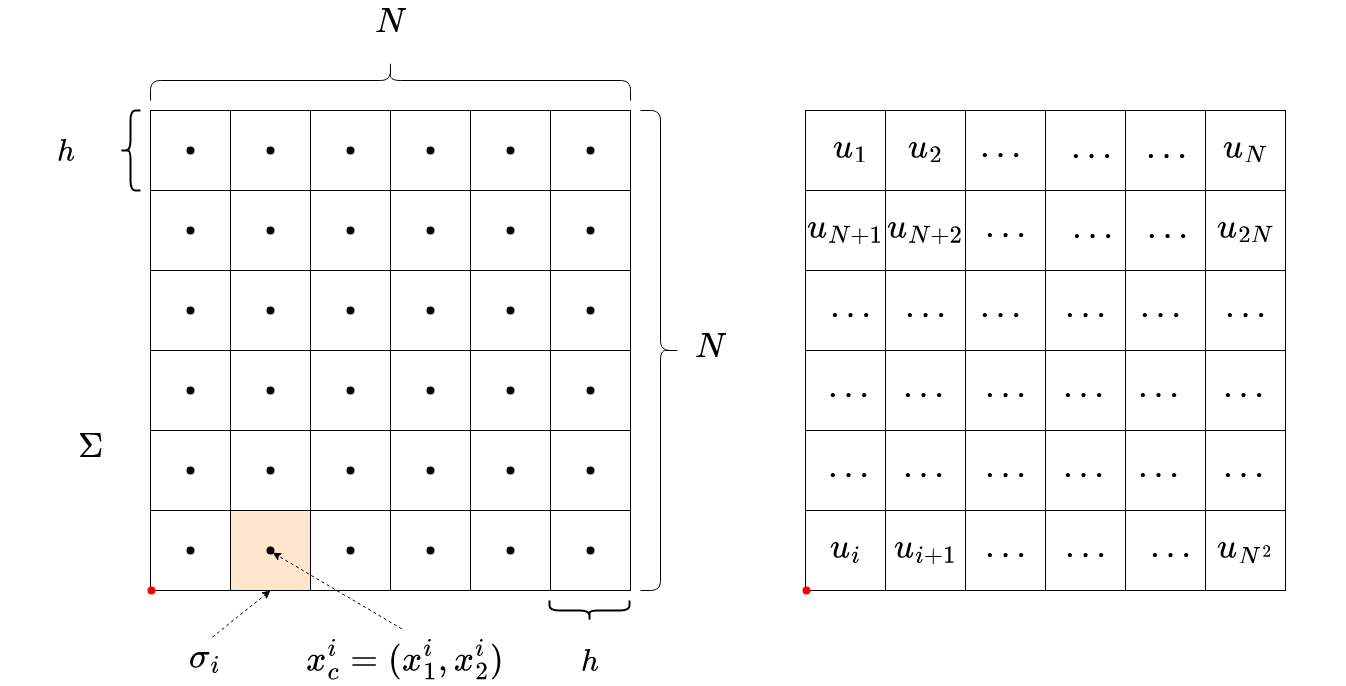
\includegraphics{diplom-Дискретизация двухмерной задачи.drawio(1).png}
\caption{Дискретизация двумерной квадратной области}
\end{figure}

с одинаковой мерой \(\mu(\sigma_i) = h^2\).

\begin{enumerate}
\def\labelenumi{\arabic{enumi}.}
\setcounter{enumi}{2}
\tightlist
\item
  Решить интегрального уравнения Фредгольма 2-го рода в двумерном случае
  с использованием метода коллокаций при \(N = 10, 20, 30, 40\) при
  помощи метода градиентного спуска, двухшагового метода градиентного
  спуска и метода биспоряженных градиентнов.
\end{enumerate}

\textbf{Постановка задачи:}

\[
U(x) + \int_{\Sigma} K(x, y)U(y)dy = f(x), \ \ x,y \in \mathbb{R}^2
\]

\begin{itemize}
\tightlist
\item
  ядро интегрального уравнения:
\end{itemize}

\[
K(x, y) = \frac{1}{4\cdot \pi \cdot |x - y|} = \frac{1}{4\cdot \pi \cdot \sqrt{(x_1 - y_1)^2 + (x_2 - y_2)^2}}, \ \ x = (x_1, x_2), \ \ y = (y_1, y_2),
\] - внешняя функция

\[
f(x) = sin(x_1) + cos(x_2)
\]

\textbf{Дискретизация уравнения:}

Уравнение в дискретном случае для метода коллокаций можно записать
следующим образом:

\[
U(x_i) + \sum_{j = 1, j\ne i}^{N^2}\int_{\sigma_j} K(x_i, y)U(y) dy = f(x_i), \ i = 1, 2, \dots, N^2,
\]

или же переписав в более удобном виде:

\[
U_i + \sum_{j = 1, j\ne i}^{N^2} K(x_i, x_j) \cdot U_j \cdot h^2 = sin(x_1^i) + cos(x_2^i), \ i = 1, 2, \dots, N^2,
\]

Получить задачу решения СЛАУ относительно неизвестного вектора \(u\):

\[
Au = f, \quad A = I + K\cdot h^2, \quad K = k_{ij} = \left\{ \begin{matrix}0, & i = j\\ \frac{1}{4 \cdot \pi \cdot |x_i - x_j|}, & i\ne j\end{matrix} \right. ,\quad f = f_i = sin(x_1^i) + cos(x_2^j).
\]

\begin{enumerate}
\def\labelenumi{\arabic{enumi}.}
\setcounter{enumi}{3}
\item
  Удостовериться в одинаковости результатов решения уравнения различными
  итерационными методами при разных значениях количества дискретных
  разбиений поверхности.
\item
  Для каждого итерационного метода показать количество умножений матрицы
  на вектор, потребовавшегося для решения задачи при различных \(N\).
  Составить сравнительную таблицу результатов.
\item
  Визуализировать результат решения задачи на двумерной плоскости в виде
  тепловой карты (figure 1, figure 2):
\end{enumerate}

\begin{figure}
\centering
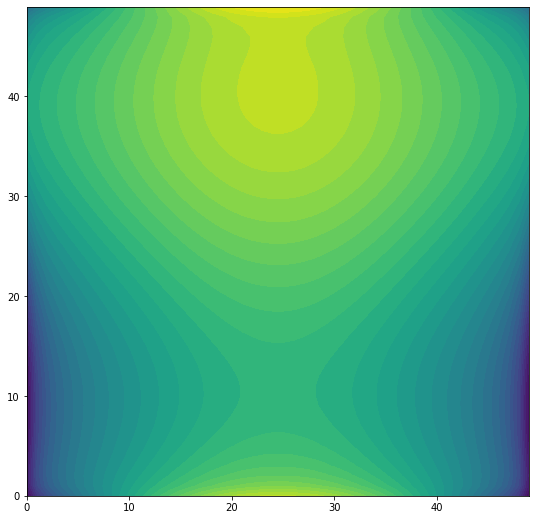
\includegraphics{2dFredholm.png}
\caption{Визуализация решения тепловой картой}
\end{figure}

\end{document}
